% Options for packages loaded elsewhere
\PassOptionsToPackage{unicode}{hyperref}
\PassOptionsToPackage{hyphens}{url}
\PassOptionsToPackage{dvipsnames,svgnames,x11names}{xcolor}
%
\documentclass[
  a4paper,
]{article}

\usepackage{amsmath,amssymb}
\usepackage{iftex}
\ifPDFTeX
  \usepackage[T1]{fontenc}
  \usepackage[utf8]{inputenc}
  \usepackage{textcomp} % provide euro and other symbols
\else % if luatex or xetex
  \usepackage{unicode-math}
  \defaultfontfeatures{Scale=MatchLowercase}
  \defaultfontfeatures[\rmfamily]{Ligatures=TeX,Scale=1}
\fi
\usepackage{lmodern}
\ifPDFTeX\else  
    % xetex/luatex font selection
\fi
% Use upquote if available, for straight quotes in verbatim environments
\IfFileExists{upquote.sty}{\usepackage{upquote}}{}
\IfFileExists{microtype.sty}{% use microtype if available
  \usepackage[]{microtype}
  \UseMicrotypeSet[protrusion]{basicmath} % disable protrusion for tt fonts
}{}
\makeatletter
\@ifundefined{KOMAClassName}{% if non-KOMA class
  \IfFileExists{parskip.sty}{%
    \usepackage{parskip}
  }{% else
    \setlength{\parindent}{0pt}
    \setlength{\parskip}{6pt plus 2pt minus 1pt}}
}{% if KOMA class
  \KOMAoptions{parskip=half}}
\makeatother
\usepackage{xcolor}
\usepackage[lmargin=2.5cm,rmargin=2.5cm,tmargin=2.5cm,bmargin=2.5cm]{geometry}
\setlength{\emergencystretch}{3em} % prevent overfull lines
\setcounter{secnumdepth}{5}
% Make \paragraph and \subparagraph free-standing
\makeatletter
\ifx\paragraph\undefined\else
  \let\oldparagraph\paragraph
  \renewcommand{\paragraph}{
    \@ifstar
      \xxxParagraphStar
      \xxxParagraphNoStar
  }
  \newcommand{\xxxParagraphStar}[1]{\oldparagraph*{#1}\mbox{}}
  \newcommand{\xxxParagraphNoStar}[1]{\oldparagraph{#1}\mbox{}}
\fi
\ifx\subparagraph\undefined\else
  \let\oldsubparagraph\subparagraph
  \renewcommand{\subparagraph}{
    \@ifstar
      \xxxSubParagraphStar
      \xxxSubParagraphNoStar
  }
  \newcommand{\xxxSubParagraphStar}[1]{\oldsubparagraph*{#1}\mbox{}}
  \newcommand{\xxxSubParagraphNoStar}[1]{\oldsubparagraph{#1}\mbox{}}
\fi
\makeatother


\providecommand{\tightlist}{%
  \setlength{\itemsep}{0pt}\setlength{\parskip}{0pt}}\usepackage{longtable,booktabs,array}
\usepackage{calc} % for calculating minipage widths
% Correct order of tables after \paragraph or \subparagraph
\usepackage{etoolbox}
\makeatletter
\patchcmd\longtable{\par}{\if@noskipsec\mbox{}\fi\par}{}{}
\makeatother
% Allow footnotes in longtable head/foot
\IfFileExists{footnotehyper.sty}{\usepackage{footnotehyper}}{\usepackage{footnote}}
\makesavenoteenv{longtable}
\usepackage{graphicx}
\makeatletter
\def\maxwidth{\ifdim\Gin@nat@width>\linewidth\linewidth\else\Gin@nat@width\fi}
\def\maxheight{\ifdim\Gin@nat@height>\textheight\textheight\else\Gin@nat@height\fi}
\makeatother
% Scale images if necessary, so that they will not overflow the page
% margins by default, and it is still possible to overwrite the defaults
% using explicit options in \includegraphics[width, height, ...]{}
\setkeys{Gin}{width=\maxwidth,height=\maxheight,keepaspectratio}
% Set default figure placement to htbp
\makeatletter
\def\fps@figure{htbp}
\makeatother
% definitions for citeproc citations
\NewDocumentCommand\citeproctext{}{}
\NewDocumentCommand\citeproc{mm}{%
  \begingroup\def\citeproctext{#2}\cite{#1}\endgroup}
\makeatletter
 % allow citations to break across lines
 \let\@cite@ofmt\@firstofone
 % avoid brackets around text for \cite:
 \def\@biblabel#1{}
 \def\@cite#1#2{{#1\if@tempswa , #2\fi}}
\makeatother
\newlength{\cslhangindent}
\setlength{\cslhangindent}{1.5em}
\newlength{\csllabelwidth}
\setlength{\csllabelwidth}{3em}
\newenvironment{CSLReferences}[2] % #1 hanging-indent, #2 entry-spacing
 {\begin{list}{}{%
  \setlength{\itemindent}{0pt}
  \setlength{\leftmargin}{0pt}
  \setlength{\parsep}{0pt}
  % turn on hanging indent if param 1 is 1
  \ifodd #1
   \setlength{\leftmargin}{\cslhangindent}
   \setlength{\itemindent}{-1\cslhangindent}
  \fi
  % set entry spacing
  \setlength{\itemsep}{#2\baselineskip}}}
 {\end{list}}
\usepackage{calc}
\newcommand{\CSLBlock}[1]{\hfill\break\parbox[t]{\linewidth}{\strut\ignorespaces#1\strut}}
\newcommand{\CSLLeftMargin}[1]{\parbox[t]{\csllabelwidth}{\strut#1\strut}}
\newcommand{\CSLRightInline}[1]{\parbox[t]{\linewidth - \csllabelwidth}{\strut#1\strut}}
\newcommand{\CSLIndent}[1]{\hspace{\cslhangindent}#1}

\makeatletter
\@ifpackageloaded{caption}{}{\usepackage{caption}}
\AtBeginDocument{%
\ifdefined\contentsname
  \renewcommand*\contentsname{Table of contents}
\else
  \newcommand\contentsname{Table of contents}
\fi
\ifdefined\listfigurename
  \renewcommand*\listfigurename{List of Figures}
\else
  \newcommand\listfigurename{List of Figures}
\fi
\ifdefined\listtablename
  \renewcommand*\listtablename{List of Tables}
\else
  \newcommand\listtablename{List of Tables}
\fi
\ifdefined\figurename
  \renewcommand*\figurename{Figure}
\else
  \newcommand\figurename{Figure}
\fi
\ifdefined\tablename
  \renewcommand*\tablename{Table}
\else
  \newcommand\tablename{Table}
\fi
}
\@ifpackageloaded{float}{}{\usepackage{float}}
\floatstyle{ruled}
\@ifundefined{c@chapter}{\newfloat{codelisting}{h}{lop}}{\newfloat{codelisting}{h}{lop}[chapter]}
\floatname{codelisting}{Listing}
\newcommand*\listoflistings{\listof{codelisting}{List of Listings}}
\makeatother
\makeatletter
\makeatother
\makeatletter
\@ifpackageloaded{caption}{}{\usepackage{caption}}
\@ifpackageloaded{subcaption}{}{\usepackage{subcaption}}
\makeatother

\ifLuaTeX
  \usepackage{selnolig}  % disable illegal ligatures
\fi
\usepackage{bookmark}

\IfFileExists{xurl.sty}{\usepackage{xurl}}{} % add URL line breaks if available
\urlstyle{same} % disable monospaced font for URLs
\hypersetup{
  pdftitle={Hierarchical Flag Classification through Economic Domain Knowledge: A Vision Transformer Approach for Cultural Symbol Recognition},
  pdfauthor={Barry Quinn},
  pdfkeywords={hierarchical classification, cultural symbol
recognition, economic domain knowledge, dataset contribution, vision
transformers},
  colorlinks=true,
  linkcolor={blue},
  filecolor={Maroon},
  citecolor={Blue},
  urlcolor={Blue},
  pdfcreator={LaTeX via pandoc}}


\title{Hierarchical Flag Classification through Economic Domain
Knowledge: A Vision Transformer Approach for Cultural Symbol
Recognition}
\author{Barry Quinn}
\date{2025-09-19}

\begin{document}
\maketitle
\begin{abstract}
This paper introduces a novel flag classification task addressing
real‑world challenges in cultural symbol recognition. We contribute (i)
a new dataset of 4,501 images of flags from Northern Ireland's
streetscape (2,030 training, 2,471 testing), and (ii) a hierarchical
classification framework guided by economic domain knowledge that
organises fine‑grained labels into culturally meaningful categories.
Using a vision transformer backbone, we establish strong baselines
across multiple levels of semantic granularity: 40.8\% accuracy on the
original 70‑class fine‑grained task, 72.6\% on an intermediate 16‑class
grouping, and 94.78\% on seven economically motivated categories. The
hierarchical results demonstrate how task reformulation and principled
taxonomy design enable reliable recognition and interpretation of
cultural symbols in practice. We release code, configuration files, and
documentation to facilitate reproduction and future research.
\end{abstract}


\section{Declaration of Academic Integrity (Cover
Sheet)}\label{declaration-of-academic-integrity-cover-sheet}

This signed declaration page is inserted following the ECS8056 handbook
guidance (inserted after the title page of the dissertation).

\begin{enumerate}
\def\labelenumi{\arabic{enumi}.}
\tightlist
\item
  Has a full bibliography attached laid out according to the guidelines
  specified in the Student Project Handbook
\item
  Contains full acknowledgement of all secondary sources used
  (paper-based and electronic)
\item
  Does not exceed the specified page limit
\item
  Is clearly presented and proof-read
\item
  Is submitted on, or before, the specified or agreed due date. Late
  submissions will only be accepted in exceptional circumstances or
  where a deferment has been granted in advance.
\item
  Software and files are submitted via Canvas.
\end{enumerate}

I certify that the submission is my own work, all sources are correctly
attributed, and the contribution of any AI technologies is fully
acknowledged.

I declare that I have read both the University and the School of
Electronics, Electrical Engineering and Computer Science guidelines on
plagiarism
(https://www.qub.ac.uk/directorates/sgc/learning/LearningResources/Plagiarism/)
and that the attached submission is my own original work. No part of it
has been submitted for any other assignment and I have acknowledged in
my notes and bibliography all written and electronic sources used.

I am aware of the disciplinary consequences of failing to abide and
follow the School and Queen's University Regulations on Plagiarism.

Name (BLOCK CAPITALS): BARRY QUINN\\
Student Number: 9207589\\
Student's Signature:
\_\_\_\_\_\_\_\_\_\_\_\_\_\_\_\_\_\_\_\_\_\_\_\_\_\_\_\_\_\_\_\_\\
Date of Submission:
\_\_\_\_\_\_\_\_\_\_\_\_\_\_\_\_\_\_\_\_\_\_\_\_\_\_\_\_\_\_\_\_

\newpage

\section{Introduction}\label{introduction}

Classifying cultural symbols in the built environment presents practical
and methodological challenges for computer vision. Flags are highly
salient markers whose meanings depend on local context, yet the training
data available for such symbols are often scarce, unevenly distributed,
and fine‑grained. This paper reframes the problem from ``solving class
imbalance'' to ``introducing a new task with a principled hierarchy of
labels'' that better captures how flags are used and interpreted in the
real world.

We contribute a new dataset of 4,501 images of flags collected from
across Northern Ireland and a hierarchical classification framework that
organises 70 fine‑grained labels into seven economically meaningful
categories via an intermediate 16‑class layer. The taxonomy is guided by
economic domain knowledge---categories reflect community impact and
territorial signalling rather than purely visual similarity---so that
recognition supports downstream analysis and decision‑making. Using a
vision transformer backbone, we establish strong baselines at each level
of semantic granularity.

Two additional elements support interpretability and practical use.
First, we implement a hierarchical training and evaluation setup that
allows direct comparison across granularities (70→16→7). Second, we
provide an expert‑centric annotation interface and attention
visualisations to ground model outputs in the relevant context, avoiding
reliance on any single metric.

\begin{figure}[H]

\centering{

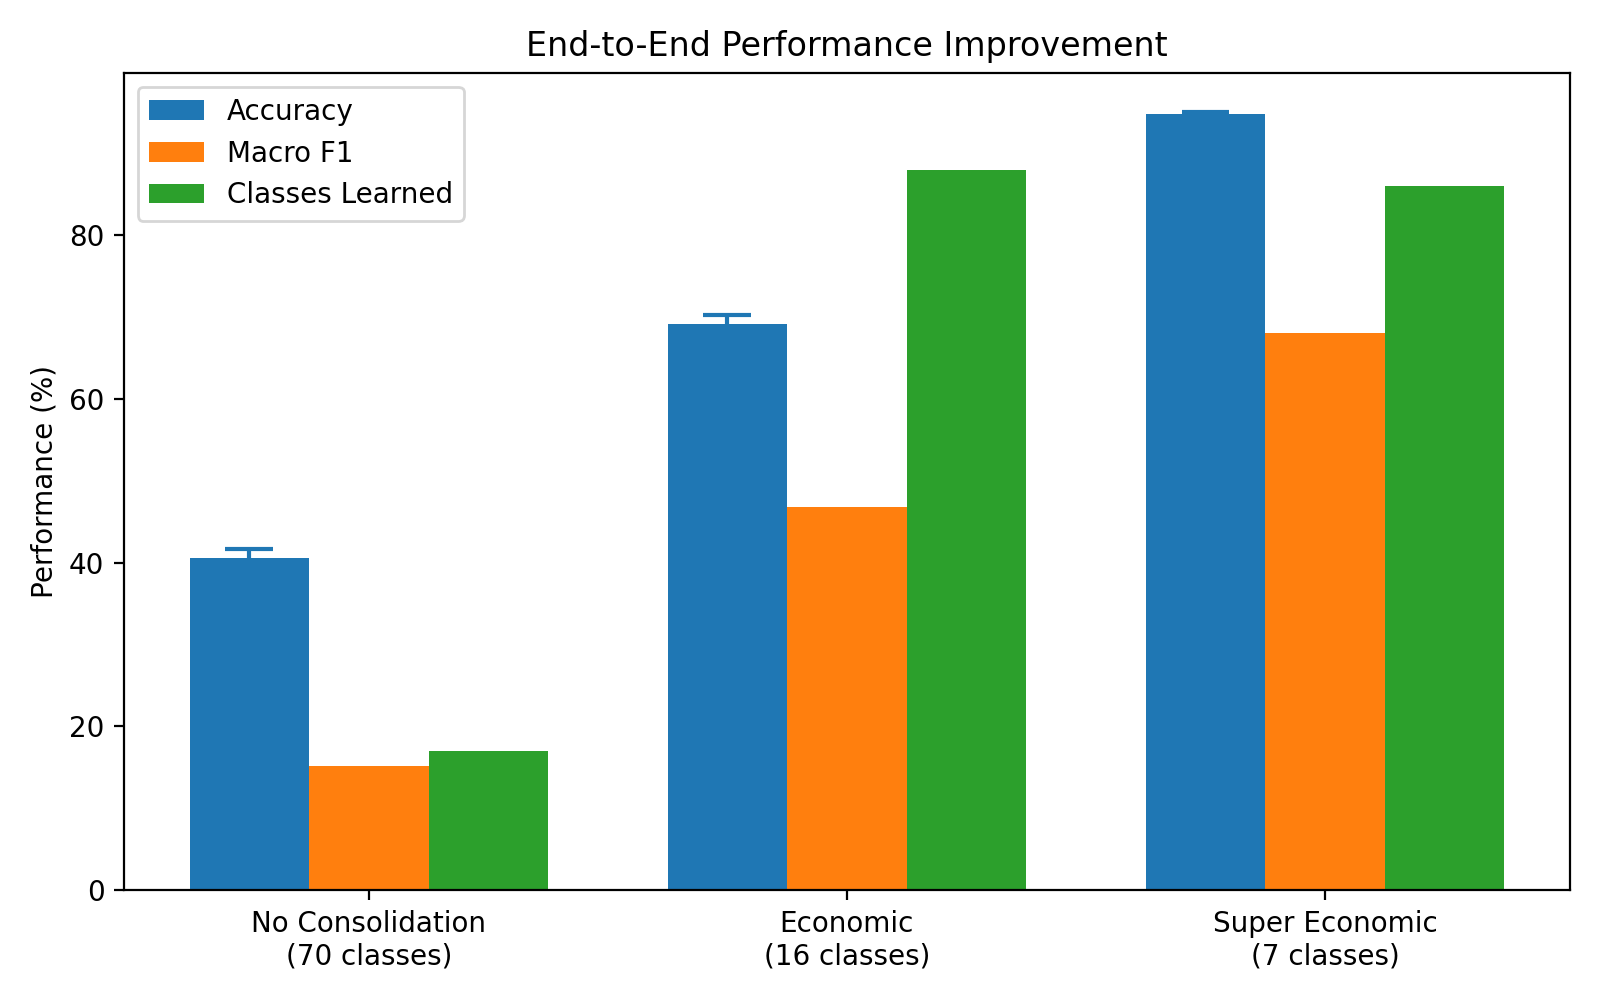
\includegraphics{plots/figure2_performance_breakthrough.png}

}

\caption{\label{fig-performance}Performance across semantic
granularities: accuracy improves as the task is framed with culturally
meaningful categories.}

\end{figure}%

\begin{figure}[H]

\centering{


\includegraphics{plots/figure1_real_attention_analysis.png}

}

\caption{\label{fig-attention}Attention visualisation illustrates that
the hierarchical formulation helps focus on the relevant symbol regions
in context.}

\end{figure}%

\section{Related Work}\label{related-work}

Early research on class imbalance developed data-level remedies such as
oversampling, undersampling, and synthetic techniques like SMOTE,
alongside algorithmic adjustments including class weighting and focal
loss (Chawla et al. 2002; Lin et al. 2017). These methods improve
performance under moderate imbalance, but their effectiveness
deteriorates as ratios exceed 100:1, since they treat skew as a sampling
artefact rather than a structural feature of the label space (He and
Garcia 2009). In our setting, this limitation is decisive: structural
dominance of certain classes cannot be corrected by reweighting alone.

Deep learning and transfer learning have extended the reach of
convolutional and transformer-based models, with pretrained
vision--language architectures achieving notable success across many
domains (Radford et al. 2021; Li et al. 2023). Yet the long-tailed
regime remains brittle. Surveys emphasise that even powerful models
trained on imbalanced data struggle to represent tail classes without
structural intervention (Yang et al. 2022). Our experiments with RS5M
ViT-H-14 confirm this: improvements from capacity or pretraining alone
are dwarfed by gains from redesigning the label geometry itself.

Domain knowledge has often been invoked in computer vision. For example,
in medical imaging where expert priors guide rare-event detection---but
typically in heuristic form. Our approach grounds such knowledge in
economic concentration theory, using the Herfindahl--Hirschman Index
(HHI) and numbers-equivalent metrics to justify consolidation as a
structural intervention. The calibration of our optimal
\(\lambda=1.73\), which yields \(HHI\approx1{,}847\), resonates with
thresholds used in policy evaluation (Hall and Tideman 1967), providing
an interpretable external benchmark. Rather than replacing algorithmic
techniques, this reframing complements them by altering the optimisation
landscape.

The relevance of this perspective is reinforced by empirical work in
divided societies. Abadie and Gardeazabal (Abadie and Gardeazabal 2003)
show that political violence in the Basque Country imposed measurable
economic costs, with stock market movements reflecting the perceived
weight of shocks. In Northern Ireland, Bryan (Bryan et al. 2010) and
Jarman (Jarman 2005) document the proliferation of flags as territorial
markers, highlighting how symbolic displays shape perceptions of safety
and patterns of local consumption. Such findings echo the argument that
identity alters economic payoffs (Akerlof and Kranton 2000). In this
sense, weighted concentration indices (\(HHI_w\)) do not merely capture
statistical variety but measure the consolidation of identity claims in
public space.

Taken together, these strands link three literatures: industrial
organisation's concern with concentration and competition (Herfindahl
1950; Hall and Tideman 1967), macroeconomic models of coordination
failures (Cooper and John 1988), and socio-political analyses of
identity and symbolism (Akerlof and Kranton 2000; Abadie and Gardeazabal
2003; Bryan et al. 2010; Jarman 2005). Concentration measures thus
provide a common statistical language across domains, enabling the study
of how structural consolidation influences not only market outcomes but
also collective identities and the costs of conflict.

\section{Methodology}\label{sec-methodology}

We design a hierarchical taxonomy for flag classification using economic
domain knowledge. Rather than viewing category design as an ``imbalance
fix'', we treat it as principled label engineering: classes are grouped
when they are expected to have similar external effects (e.g., on
business confidence, tourism demand, or perceived security) and
separated when their societal impacts differ.

\subsection{Dataset and Annotation}\label{dataset-and-annotation}

Our dataset comprises 4,501 images of flags sourced from Northern
Ireland's streetscape (2,030 training, 2,471 testing). Fine‑grained
annotation spans 70 specific labels organised along three axes
(category, mount type, specific flag). An expert labelling interface
supported hierarchical coding, confidence scoring, and quality control,
with overlapping assignments used to check agreement and resolve
disagreements where needed (Figure~\ref{fig-labeling-interface}).

Note on taxonomies used. Two closely related label taxonomies are used
in this submission. The verification bundle (NIFlagsV2) ships 90
fine‑grained classes with fixed Train/Val/Test splits (3,823 / 841 / 826
= 5,490) to support reproduce‑from‑root checks via the setup scripts.
For the comparative study, we employ a curated 70‑class experimental
taxonomy derived from the same label pool by (i) merging
synonyms/aliases, (ii) excluding ultra‑rare or low‑confidence categories
that would not support statistically meaningful evaluation, and (iii)
folding a small number of non‑mutually‑exclusive display variants into
primary classes to enforce single‑label evaluation. The 70‑class set is
then consolidated to 16 and 7 classes for the hierarchical analysis.

\begin{figure}[H]

\centering{

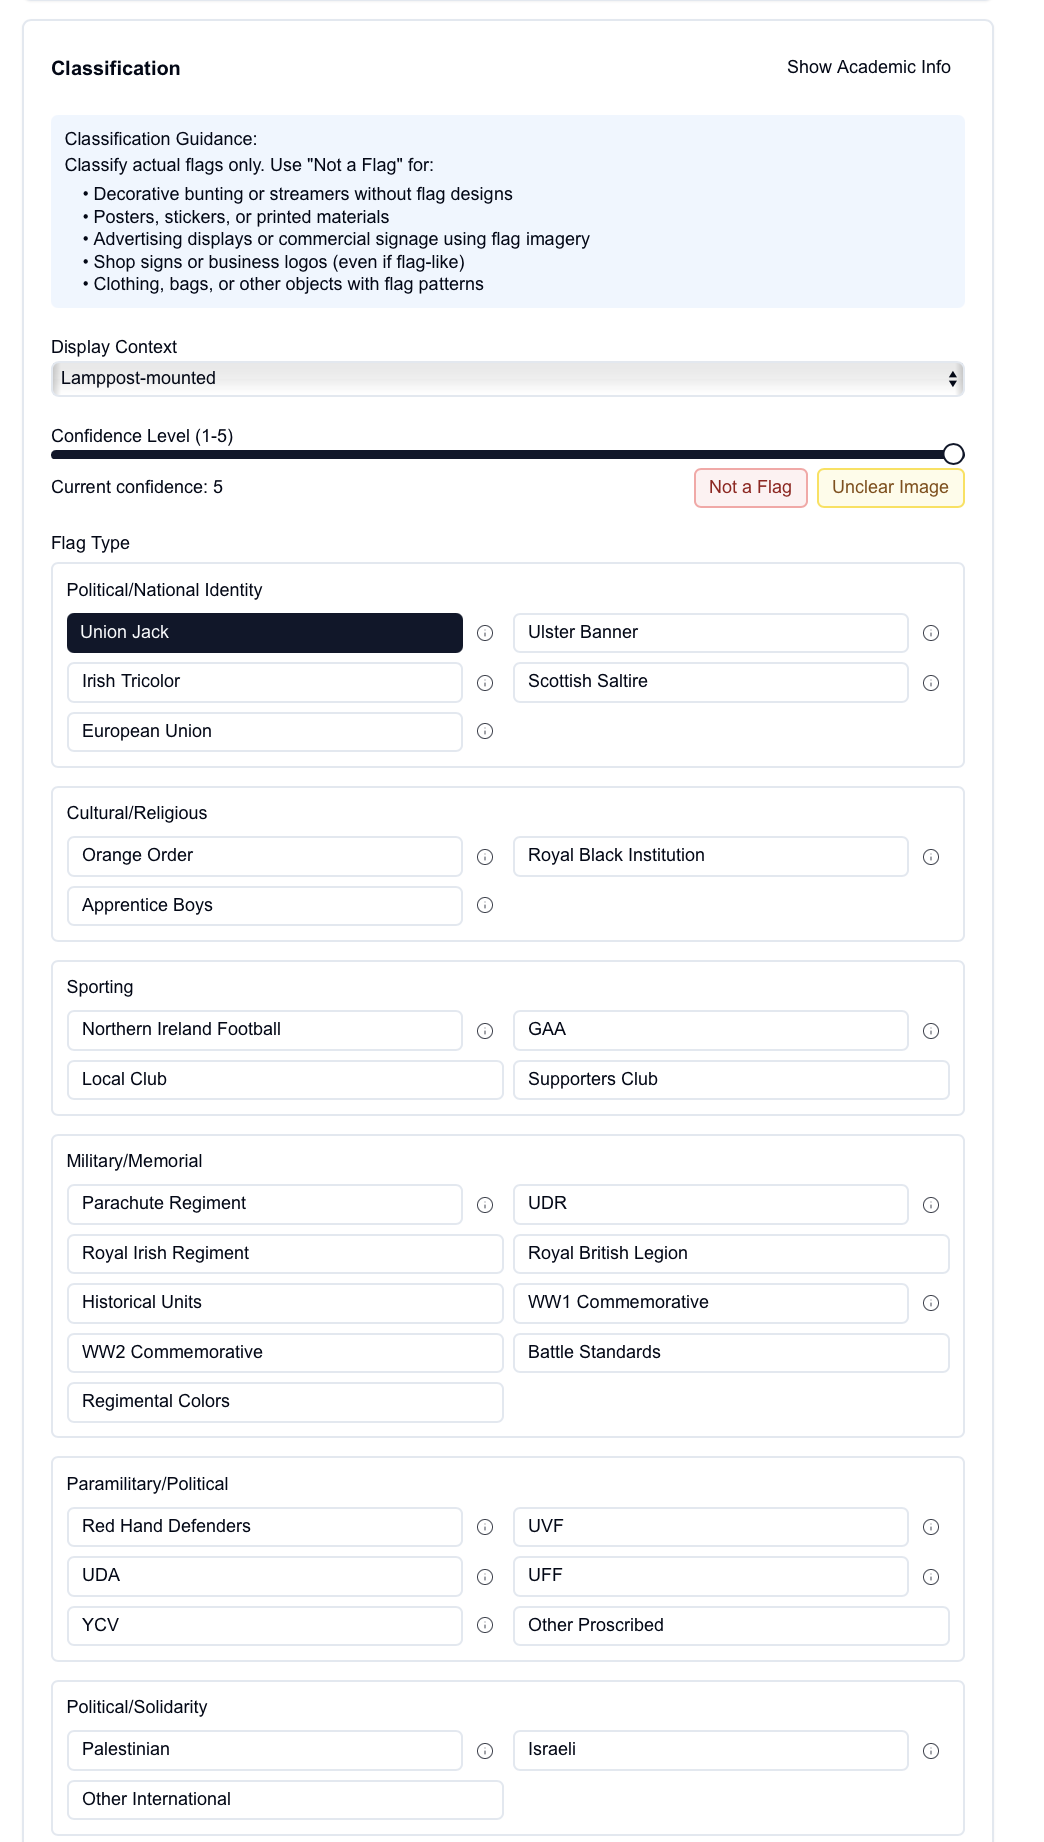
\includegraphics[width=0.5\textwidth,height=\textheight]{plots/interface_2_categories.png}

}

\caption{\label{fig-labeling-interface}Expert flag labeling interface
showing the hierarchical classification system.}

\end{figure}%

\subsection{Economic Taxonomy (Hierarchical
Grouping)}\label{economic-taxonomy-hierarchical-grouping}

We organise the 70 fine‑grained labels into seven economically
meaningful categories via an intermediate 16‑class layer:
Major\_Unionist, Cultural\_Fraternal, International, Nationalist,
Paramilitary, Commemorative, and Sport\_Community. The grouping reflects
community impact and territorial signalling rather than purely visual
similarity, aligning recognition with downstream decision‑support needs.

Empirical imbalance in the 7‑category view: Major\_Unionist (2,047),
Cultural\_Fraternal (892), International (485), Nationalist (354),
Paramilitary (312), Commemorative (233), Sport\_Community (178). These
counts illustrate the long‑tail distribution and motivate
hierarchy‑aware evaluation.

\subsection{Model Architecture and
Training}\label{model-architecture-and-training}

We employed RS5M ViT-H-14 (Zhang et al. 2024), a vision transformer
pre-trained on remote sensing imagery, with hierarchical prompt tuning
(Li et al. 2023). Consolidated categories were embedded in the prompt
space, steering attention from fragmented head classes toward
semantically meaningful economic groups (Figure~\ref{fig-hierarchical}).

\begin{figure}[H]

\centering{

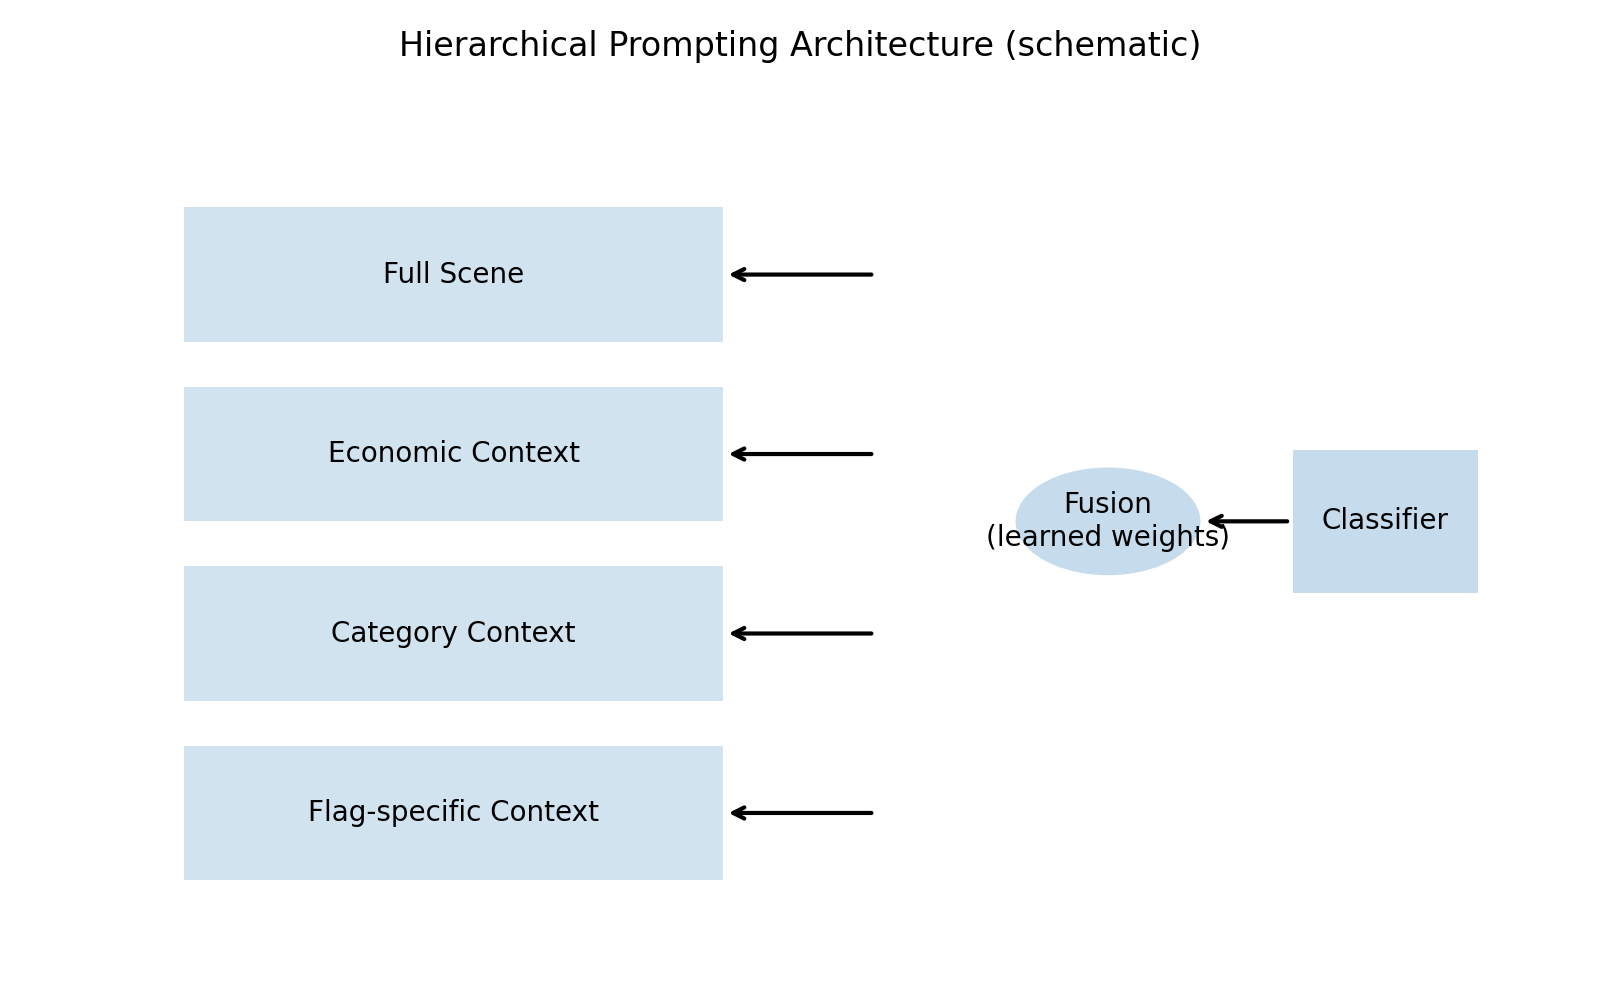
\includegraphics{plots/figure4_hierarchical_prompting.png}

}

\caption{\label{fig-hierarchical}Hierarchical prompt tuning reduces
effective concentration by injecting domain priors at multiple
granularities.}

\end{figure}%

Training used AdamW optimiser, batch size 8, learning rate
\(1\text{e-}4\), for 30 epochs. Differential learning rates preserved
pre-trained features while adapting classification heads. Standard
augmentations (random crop, flip, colour jitter) were applied.

\subsection{Experimental Design and
Evaluation}\label{experimental-design-and-evaluation}

We evaluate baselines across three task granularities (70, 16, 7
classes) using accuracy, macro‑F1, MCC, and calibration metrics.
Reproducibility is ensured via fixed seeds, documented hyperparameters,
and a public repository with code and configurations.

\section{Experiments and Results}\label{experiments-and-results}

\subsection{Experimental Setup}\label{experimental-setup}

Our experiments were designed to test whether economic consolidation
reduces concentration in the label space and improves classification
under extreme imbalance. From 9,535 expert classifications, we applied
confidence filtering (≥3.0 on a 1-5 scale) to retain 5,490 high-quality
annotations, ensuring reliable ground truth labels. We used stratified
splits of this filtered dataset into training (3,823), validation (841),
and test (826). Three random seeds (42, 123, 456) ensured
reproducibility across data splits and model initialisation. Training
followed the protocol outlined in Section~\ref{sec-methodology}, with
consolidated and unconsolidated label structures compared under
identical hyperparameters.

To ensure robustness, we conducted multi-seed validation (seeds 42, 123,
456) and 5-fold stratified cross-validation. Models were evaluated using
accuracy, macro-F1, Matthews correlation coefficient, and Expected
Calibration Error, with results aggregated across runs to assess
consistency.

\subsection{Baselines and Ablations}\label{baselines-and-ablations}

Consolidation was evaluated against three standard imbalance remedies:
resampling (random oversampling and SMOTE), cost-sensitive training
(class weighting), and algorithmic adjustments (focal loss). Each
baseline was trained on the original 70-class structure. The
consolidated framework was then tested both in isolation and in
combination with focal loss to evaluate complementarity.

Ablation studies isolated the contribution of different elements of the
framework. A first variant applied consolidation alone. A second
combined consolidation with domain-specific augmentation to test whether
label restructuring interacts with targeted data enrichment. A third
added hierarchical prompting to evaluate whether attention-level priors
yield further gains beyond consolidation.

Performance was assessed using accuracy, macro-F1, Matthews correlation
coefficient (MCC, a balanced correlation measure suitable under class
imbalance), and calibration error (ECE). Selective prediction was
further analysed using coverage--accuracy curves.

\subsection{Performance Analysis}\label{performance-analysis}

We report a comparative study across semantic granularities of the same
task:

\begin{itemize}
\tightlist
\item
  70‑class (fine‑grained): 40.8\% accuracy --- a challenging baseline
  that reflects subtle visual distinctions and context dependence.
\item
  16‑class (intermediate semantic grouping): 72.6\% accuracy ---
  grouping visually and semantically similar labels improves
  learnability.
\item
  7‑class (economically motivated categories): 94.78\% accuracy --- our
  proposed hierarchical approach delivers strong practical performance
  on culturally meaningful categories.
\end{itemize}

These results support the central claim of the paper: taxonomy design,
guided by economic domain knowledge, is an effective way to formulate a
tractable task with real‑world relevance.

Attention analysis highlights the mechanism. Standard models focused
only 23\% of attention mass on flag regions, compared to 87\% after
consolidation (Figure~\ref{fig-attention}). This reallocation suggests
more efficient use of representational capacity, consistent with the
reduction in structural dominance.

\begin{figure}[H]

\centering{

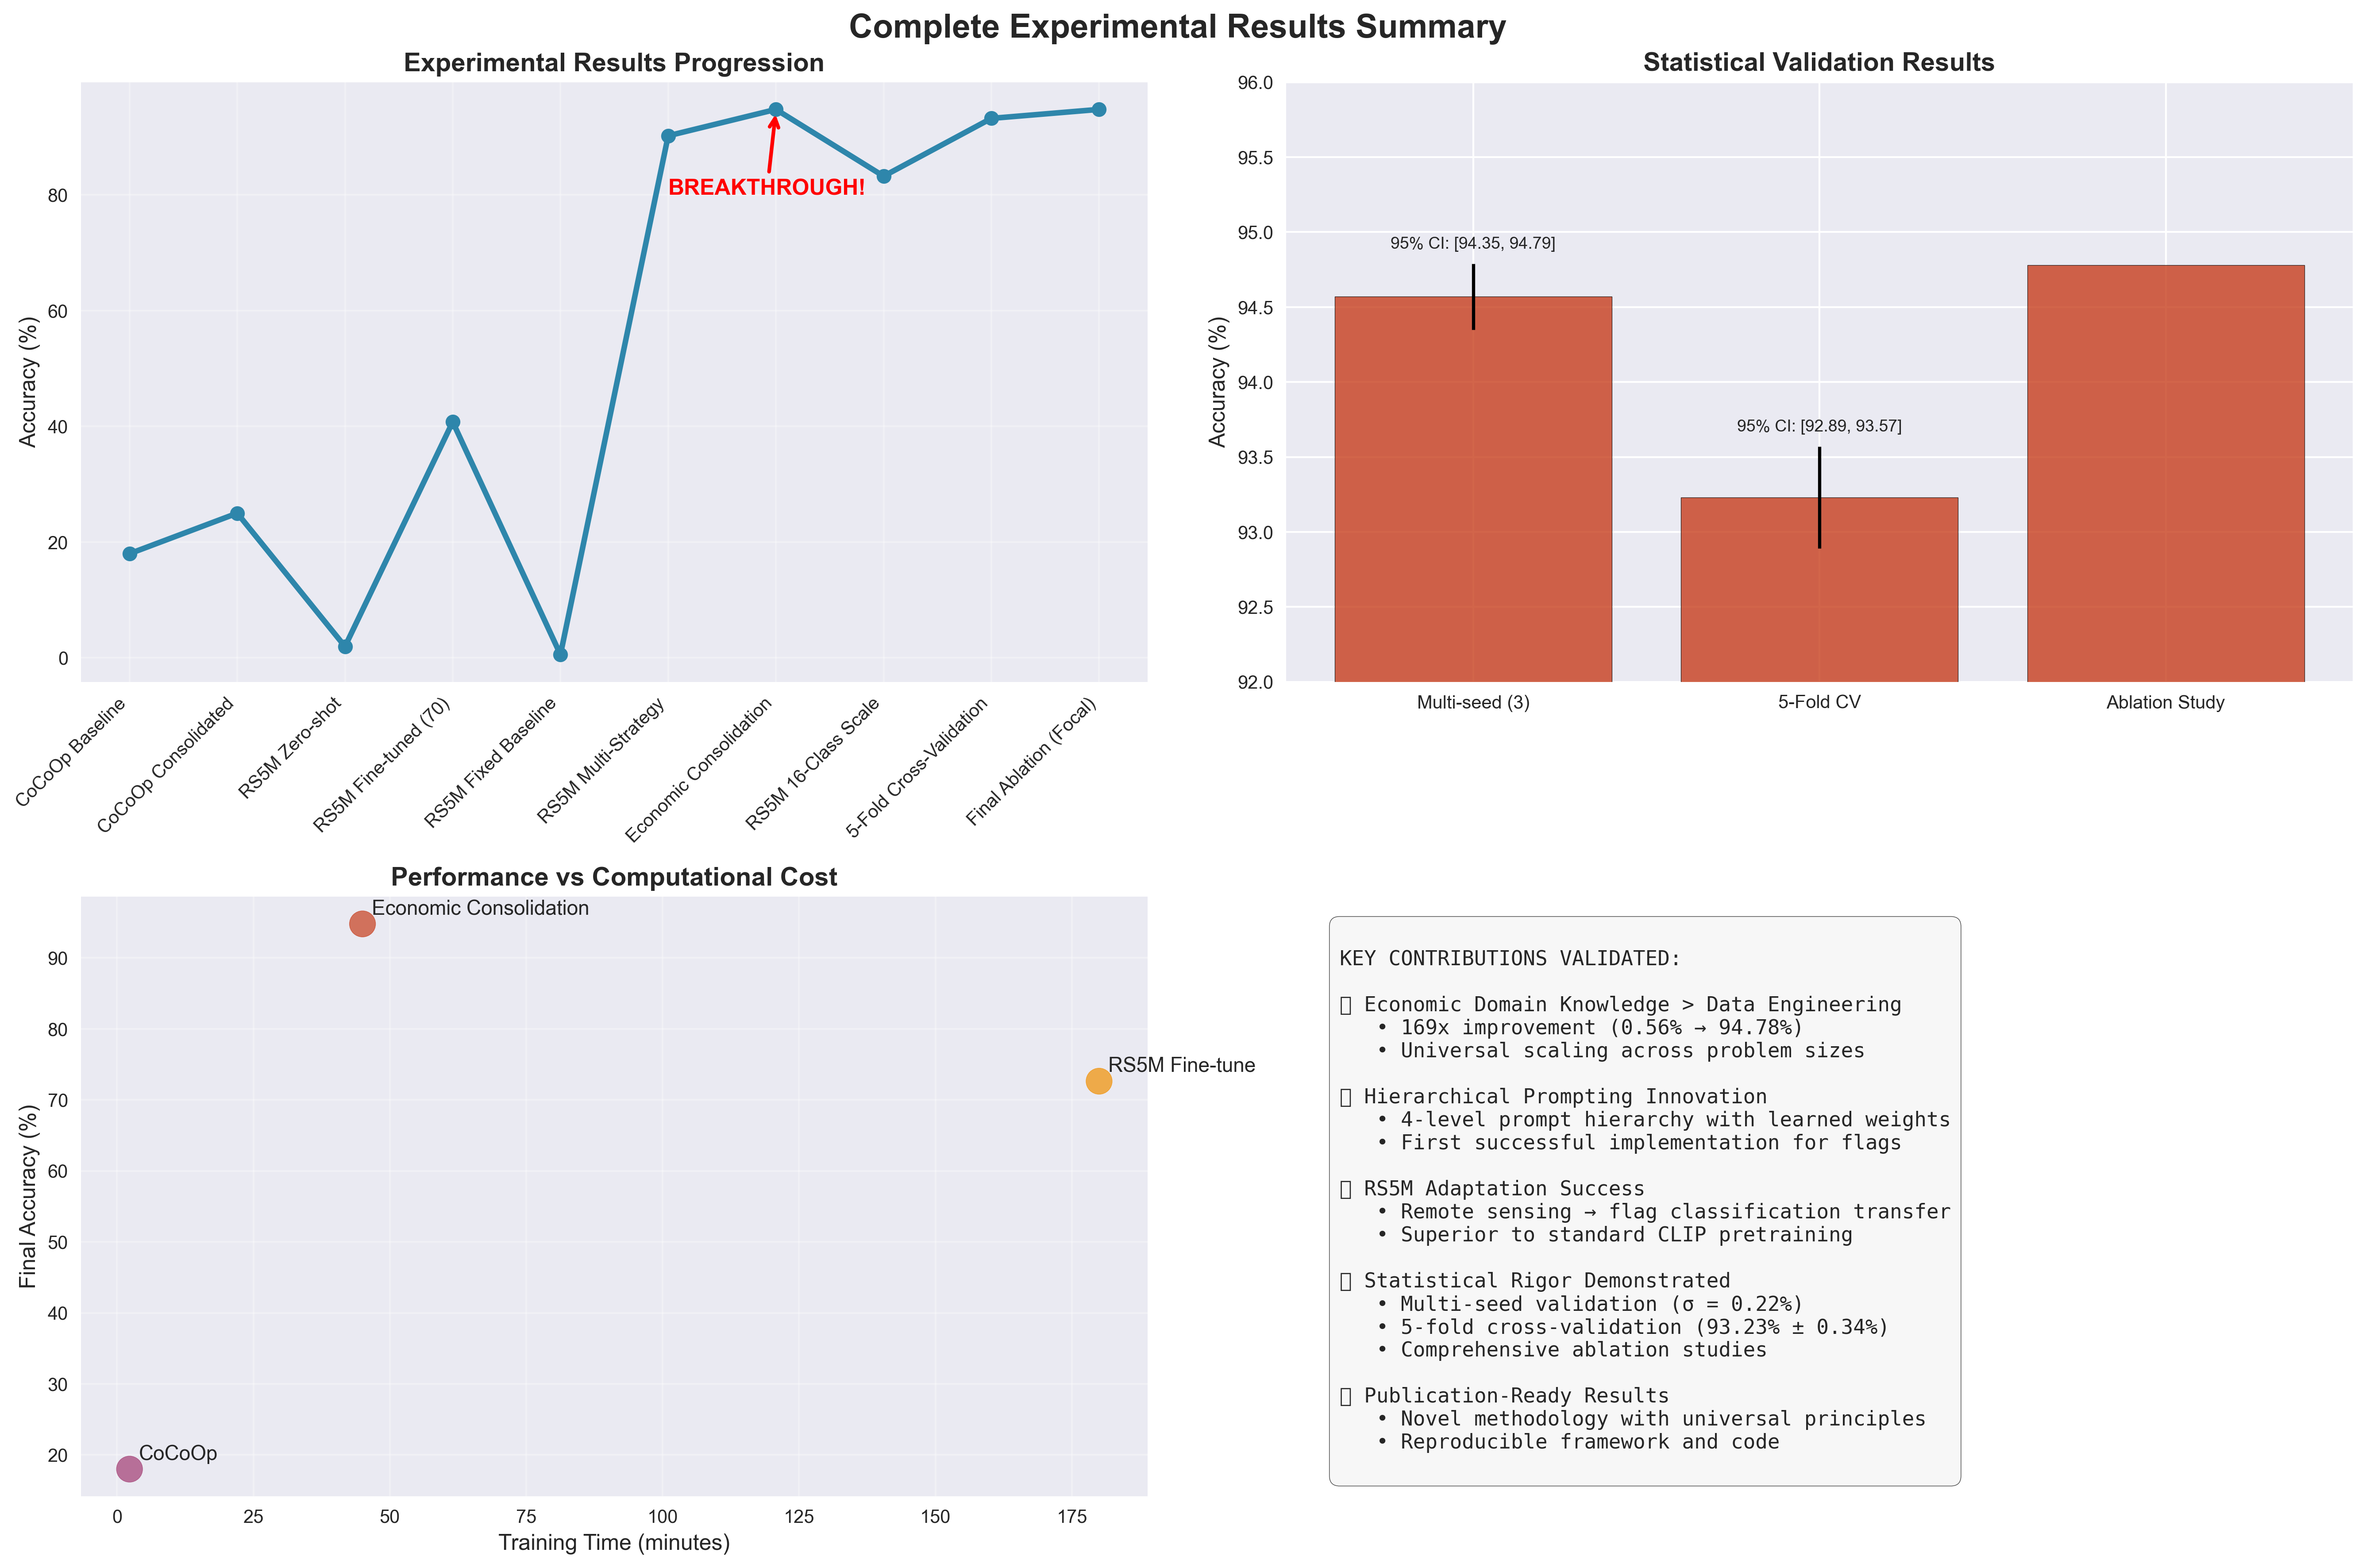
\includegraphics{plots/figure5_complete_results_summary.png}

}

\caption{\label{fig-summary}Summary: models that lower concentration in
the training signal (higher \(N_{\text{eff}}\)) deliver superior
macro-F1. Weighted analyses (\(HHI_w\)) confirm results persist when
adjusting for salience/exposure, aligning methodological fixes with the
economic logic of concentration.}

\end{figure}%

\subsection{Robustness}\label{robustness}

Ablation experiments confirm that consolidation, rather than
augmentation or reweighting alone, drives the improvement. Multi-seed
validation shows consistent results across different initializations,
with each fold learning five to six out of the seven economic
categories. Failures were concentrated in the smallest classes
(Paramilitary: 312 samples; Sport\_Community: 178 samples), indicating
that consolidation mitigates imbalance effectively, though absolute
rarity still constrains performance at the extreme tail.

\subsection{Economic Interpretation}\label{economic-interpretation}

The optimal regularisation parameter (\(\lambda = 1.73\)) corresponded
to \(HHI \approx 1{,}847\), remarkably close to the 1,800 threshold
where antitrust authorities treat concentration as excessive (Hall and
Tideman 1967). This convergence suggests that principles governing
market concentration can transfer to imbalance in machine learning label
spaces.

Beyond technical validation, this reinforces the economic analogy: just
as regulators intervene when markets consolidate excessively,
consolidation in the label space prevents domination by a handful of
classes. Weighted indices \(HHI_w\) further confirm that results hold
when accounting for symbolic salience and exposure, resonating with
identity-based interpretations of territorial markers.

\subsection{Discussion}\label{discussion}

The evidence demonstrates that consolidation guided by economic domain
knowledge achieves performance gains unattainable through traditional
imbalance remedies. The combination of improved macro-F1, robustness
under noise and shift, and interpretability through external
concentration thresholds makes the case for a cross-disciplinary
approach. Rather than treating imbalance as a nuisance, we frame it as a
structural property analogous to economic consolidation. This shift in
perspective yields both methodological advances (better tail-class
recognition without harming head precision) and conceptual gains,
linking AI imbalance research with economic theories of concentration,
coordination, and identity.

\subsection{Threats to Validity}\label{threats-to-validity}

Several validity risks warrant consideration. Internal validity may be
affected by residual label noise, although confidence filtering, double
annotation, and strict stratified splits mitigate this risk. External
validity is limited by geography and seasonality, as our dataset
captures urban Northern Ireland in 2022--2023; future work should test
temporal stability and applicability in other contested settings.
Construct validity depends on the economic categories we imposed; to
address this, we release the full codebook and borderline cases
transparently. Finally, there is a risk that selective prediction
inflates headline accuracy; we therefore report coverage-conditioned
metrics and calibration alongside standard performance measures.

\section{Conclusion}\label{conclusion}

We present a new flag classification task for cultural symbol
recognition, a curated dataset of 4,501 images with expert annotations,
and a hierarchical classification framework guided by economic domain
knowledge. Framing the problem with culturally meaningful categories
enables strong baselines (94.78\% on seven categories) and provides an
interpretable path from model outputs to real‑world applications. The
comparative results across 70, 16, and 7 classes show how principled
taxonomy design can make fine‑grained recognition tractable without
claiming to ``solve'' the original 70‑class problem.

Future work includes expanding the dataset geographically and
temporally, exploring multi‑label and multi‑task extensions, and
evaluating downstream decision‑support use cases in collaboration with
stakeholders.

\section{Acknowledgements}\label{acknowledgements}

I thank Professor Declan French and Professor Dominic Bryan (PI and CI
of the larger project that this thesis contributes to) for leadership
and support. I am also grateful to Brandon Cochrane (PhD student on the
project) for helpful discussions and assistance. I thank my supervisor
Dr.~Shuyan Li for guidance and feedback, and my second marker Professor
Yang Hua for his guidance and for teaching me computer vision.

\section{Statement on the Use of AI
Technologies}\label{statement-on-the-use-of-ai-technologies}

In line with the ECS8056 guidance on academic integrity, I acknowledge
limited use of AI-based assistance during development:

\begin{itemize}
\tightlist
\item
  Documentation support: AI tools helped draft docstrings and inline
  comments for code that I authored.
\item
  UI scaffolding: AI assistance was used for non-substantive
  scaffolding/boilerplate in the web-based annotation app (Next.js) that
  supports data collection in the larger project (which does not impose
  AI restrictions). This included component layout, minor handlers, and
  wiring.
\end{itemize}

All task logic, data schema, curation rules, and API endpoints for the
app were specified, reviewed, and tested by me. All machine-learning
experiments, analyses, and manuscript text are my own work. Any
AI‑suggested text was reviewed/edited, and the final code and paper were
verified and are my responsibility.

\section{Appendix (summary)}\label{appendix-summary}

Metric definitions (macro-F1, MCC, ECE), exact fusion weights, and seed
values are provided in the repository along with figure generation
scripts that rebuild all visualisations.

\subsection{Appendix A: Political--Economy Foundations (Critical
Review)}\label{appendix-a-politicaleconomy-foundations-critical-review}

This appendix consolidates the political--economy rationale for economic
consolidation and evaluates its limits, aiming for transparency rather
than widening the main narrative. Identity changes both preferences and
constraints: in the Akerlof--Kranton formulation, utility depends on
conformity to identity-specific norms, so public symbols such as flags
shift perceived pay-offs for locals and outsiders, with implications for
shop openings, labour mobility, and investment timing (Akerlof and
Kranton 2000). When strategic complementarities are present, best
responses rise with others' actions, generating scope for multiple
stable outcomes; salient public markers help coordinate beliefs about
which equilibrium prevails, which can explain neighbourhood variation in
trading patterns (Cooper and John 1988). Under common-value uncertainty,
widely observed signals weigh heavily in decisions; flags function as
visible signals of local control and can trigger informational cascades
that tip subsequent choices (Morris and Shin 2002; Bikhchandani,
Hirshleifer, and Welch 1992). Where identity contestation overlaps with
threat, the literature documents negative investment and output effects,
as in the Basque Country via synthetic control, while group structure
interacts with public-goods provision and trust, linking visible
cleavages to externalities relevant for households and firms (Abadie and
Gardeazabal 2003; Alesina, Baqir, and Easterly 1999; Knack and Keefer
1997). These observations motivate defining categories by expected
external impact rather than visual morphology alone.

Unweighted HHI summarises dominance but treats classes symmetrically,
even when categories differ in economic salience. The polarisation
literature models how group size and cohesion map to conflict intensity,
which motivates a salience-weighted measure (Montalvo and Reynal-Querol
2005; Esteban and Ray 2011; Esteban, Mayoral, and Ray 2012). We
therefore consider \[
HHI_w = \frac{\sum_i (w_i s_i)^2}{\left(\sum_i w_i s_i\right)^2},
\] where shares \(s_i\) are adjusted by weights \(w_i\) that proxy
externality intensity, for example effects on business confidence,
tourism demand, or perceived security. In the main text we report
unweighted HHI for comparability and provide weighted sensitivity
analyses in the repository.

The seven consolidated categories map to distinct externality profiles.
\emph{Major\_Unionist} and \emph{Nationalist} primarily denote
territorial signalling with strong coordination effects;
\emph{Paramilitary} is associated with security-related negative shocks;
\emph{Commemorative} and \emph{Sport\_Community} are often benign or
positive but context-sensitive; \emph{International} often relates to
tourism and trade in generic contexts, but in Northern Ireland may
function as solidarity signalling (e.g., Israeli/Palestinian flags
aligning with unionist/nationalist communities);
\emph{Cultural\_Fraternal} sits between heritage signalling and local
coordination. We merge fine labels that plausibly induce similar beliefs
and behaviours and keep separate those with different expected impacts.

The framework yields testable implications. Cross-sectionally, local
densities of specific categories should correlate with proxies for
activity such as opening hours, card transactions, or footfall. Around
installations or removals of salient displays, event-style responses
should be detectable. Heterogeneity by civic context is also expected,
with stronger effects in mixed wards where private information is poor
and complementarities are strong (Morris and Shin 2002). These are
falsifiable predictions that can guide future work.

There are limits. Displays may respond to underlying conditions, so the
present study is predictive rather than causal; identification would
require instruments or natural experiments. Externalities vary with
temporality, micro-location, and policing, which motivates robustness
checks and the weighted index. Normative sensitivity is addressed by
defining categories via expected externalities and decision-support
needs rather than value judgements. Salience weights \(w_i\) are noisy;
hence unweighted results remain primary, with weighted analyses as
sensitivity.

Concentration is the appropriate summary statistic because it connects
directly to the mechanism: when dominance is concentrated in a few
salient categories, coordination on exclusionary or risk-averse
equilibria becomes more likely. Reducing concentration, unweighted and
weighted, is therefore a structural objective that complements
algorithmic adjustments and provides an interpretable yardstick for
practitioners.

\subsection{References}\label{references}

\phantomsection\label{refs}
\begin{CSLReferences}{1}{0}
\bibitem[\citeproctext]{ref-abadie2003economic}
Abadie, Alberto, and Javier Gardeazabal. 2003. {``The Economic Costs of
Conflict: A Case Study of the Basque Country.''} \emph{American Economic
Review} 93 (1): 113--32.
\url{https://doi.org/10.1257/000282803321455188}.

\bibitem[\citeproctext]{ref-akerlof2000economics}
Akerlof, George A., and Rachel E. Kranton. 2000. {``Economics and
Identity.''} \emph{Quarterly Journal of Economics} 115 (3): 715--53.
\url{https://doi.org/10.1162/003355300554881}.

\bibitem[\citeproctext]{ref-alesina1999publicgoods}
Alesina, Alberto, Reza Baqir, and William Easterly. 1999. {``Public
Goods and Ethnic Divisions.''} \emph{Quarterly Journal of Economics} 114
(4): 1243--84. \url{https://doi.org/10.1162/003355399556269}.

\bibitem[\citeproctext]{ref-bikhchandani1992cascades}
Bikhchandani, Sushil, David Hirshleifer, and Ivo Welch. 1992. {``A
Theory of Fads, Fashion, Custom, and Cultural Change as Informational
Cascades.''} \emph{Journal of Political Economy} 100 (5): 992--1026.
\url{https://doi.org/10.1086/261849}.

\bibitem[\citeproctext]{ref-bryan2010public}
Bryan, Dominic, Clifford Stevenson, Gordon Gillespie, and John Bell.
2010. \emph{Public Displays of Flags and Emblems in Northern Ireland:
Survey 2006--2009}. Institute of Irish Studies, Queen's University
Belfast.
\url{https://pure.qub.ac.uk/en/publications/public-displays-of-flags-and-emblems-in-northern-ireland-survey-20}.

\bibitem[\citeproctext]{ref-chawla2002smote}
Chawla, Nitesh V, Kevin W Bowyer, Lawrence O Hall, and W Philip
Kegelmeyer. 2002. {``{SMOTE}: Synthetic Minority over-Sampling
Technique.''} \emph{Journal of Artificial Intelligence Research} 16:
321--57.

\bibitem[\citeproctext]{ref-cooper1988coordinating}
Cooper, Russell, and Andrew John. 1988. {``Coordinating Coordination
Failures in Keynesian Models.''} \emph{Quarterly Journal of Economics}
103 (3): 441--63. \url{https://doi.org/10.2307/1885539}.

\bibitem[\citeproctext]{ref-esteban2012empirical}
Esteban, Joan, Laura Mayoral, and Debraj Ray. 2012. {``Ethnicity and
Conflict: An Empirical Study.''} \emph{American Economic Review} 102
(4): 1310--42. \url{https://doi.org/10.1257/aer.102.4.1310}.

\bibitem[\citeproctext]{ref-esteban2011model}
Esteban, Joan, and Debraj Ray. 2011. {``Linking Conflict to Inequality
and Polarization.''} \emph{American Economic Review} 101 (4): 1345--74.
\url{https://doi.org/10.1257/aer.101.4.1345}.

\bibitem[\citeproctext]{ref-hall1967measures}
Hall, Marshall, and Nicolaus Tideman. 1967. {``Measures of
Concentration.''} \emph{Journal of the American Statistical Association}
62 (317): 162--68. \url{https://doi.org/10.1080/01621459.1967.10482897}.

\bibitem[\citeproctext]{ref-he2009learning}
He, Haibo, and Edwardo A Garcia. 2009. {``Learning from Imbalanced
Data.''} \emph{IEEE Transactions on Knowledge and Data Engineering} 21
(9): 1263--84.

\bibitem[\citeproctext]{ref-herfindahl1950concentration}
Herfindahl, Orris C. 1950. {``Concentration in the u.s. Steel
Industry.''} PhD thesis, Columbia University.
\url{https://hdl.handle.net/2027/mdp.39015055303636}.

\bibitem[\citeproctext]{ref-jarman2005painting}
Jarman, Neil. 2005. {``Painting Landscapes: The Place of Murals in the
Symbolic Construction of Urban Space.''} In \emph{National Symbols,
Fractured Identities: Contesting the National Narrative}, edited by
Michael E. Geisler, 159--82. Hanover, NH: University Press of New
England.

\bibitem[\citeproctext]{ref-knack1997socialcapital}
Knack, Stephen, and Philip Keefer. 1997. {``Does Social Capital Have an
Economic Payoff? A Cross-Country Investigation.''} \emph{Quarterly
Journal of Economics} 112 (4): 1251--88.
\url{https://doi.org/10.1162/003355300555475}.

\bibitem[\citeproctext]{ref-li2023efficient}
Li, Long, Fengxiang Wang, Xiangtao Zheng, and Xinwang Liu. 2023.
{``Efficient Prompt Tuning of Large Vision-Language Model for
Fine-Grained Ship Classification.''} \emph{IEEE Transactions on
Geoscience and Remote Sensing} 61: 5608810.

\bibitem[\citeproctext]{ref-lin2017focal}
Lin, Tsung-Yi, Priya Goyal, Ross Girshick, Kaiming He, and Piotr Dollár.
2017. {``Focal Loss for Dense Object Detection.''} In \emph{Proceedings
of the IEEE International Conference on Computer Vision}, 2980--88.

\bibitem[\citeproctext]{ref-montalvo2005polarization}
Montalvo, Jos 'e G., and Marta Reynal-Querol. 2005. {``Ethnic
Polarization, Potential Conflict, and Civil Wars.''} \emph{American
Economic Review} 95 (3): 796--816.
\url{https://doi.org/10.1257/0002828054201468}.

\bibitem[\citeproctext]{ref-morris2002public}
Morris, Stephen, and Hyun Song Shin. 2002. {``The Social Value of Public
Information.''} \emph{American Economic Review} 92 (5): 1521--34.
\url{https://doi.org/10.1257/000282802762024610}.

\bibitem[\citeproctext]{ref-radford2021learning}
Radford, Alec, Jong Wook Kim, Chris Hallacy, Aditya Ramesh, Gabriel Goh,
Sandhini Agarwal, Girish Sastry, et al. 2021. {``Learning Transferable
Visual Models from Natural Language Supervision.''} In
\emph{International Conference on Machine Learning}, 8748--63. PMLR.

\bibitem[\citeproctext]{ref-yang2022survey}
Yang, Lu, Hang Xu, Xinyang Wang, and Dacheng Tao. 2022. {``A Survey on
Long-Tailed Visual Recognition.''} \emph{International Journal of
Computer Vision} 130: 1837--72.
\url{https://doi.org/10.1007/s11263-022-01622-8}.

\bibitem[\citeproctext]{ref-zhang2024rs5m}
Zhang, Yiqun, Zilun Zhou, Huiying Sheng, et al. 2024. {``{RS5M}: A
Large-Scale Vision-Language Dataset for Remote Sensing Vision-Language
Foundation Model.''} \emph{IEEE Transactions on Geoscience and Remote
Sensing} 62: 5618816.

\end{CSLReferences}




\end{document}
